% Отчёт по лабораторной работе №3
% «Матрицы в 3D-графике»

\chapter{Ход выполнения работы}

\section{Задание 1. Построение куба в пространстве}

Для выполнения заданий используется код Python с библиотекой matplotlib для 3D визуализации.

\textbf{Зачем использовать четырехкомпонентный вектор?}

Четырехкомпонентный вектор (где последняя координата $w$) позволяет удобно записывать любые аффинные преобразования — такие как перенос, масштабирование и поворот — в виде одного матричного умножения. Благодаря этому все преобразования можно объединять и применять последовательно, не переходя к разным формулам для разных типов операций. После применения преобразования для получения обычных координат достаточно разделить $x$, $y$, $z$ на $w$ (если $w \neq 1$).

\textbf{Как задать другие фигуры?}

Для построения других многогранников достаточно изменить содержимое массивов координат вершин и индексов граней.

\begin{figure}[h!]
    \centering
    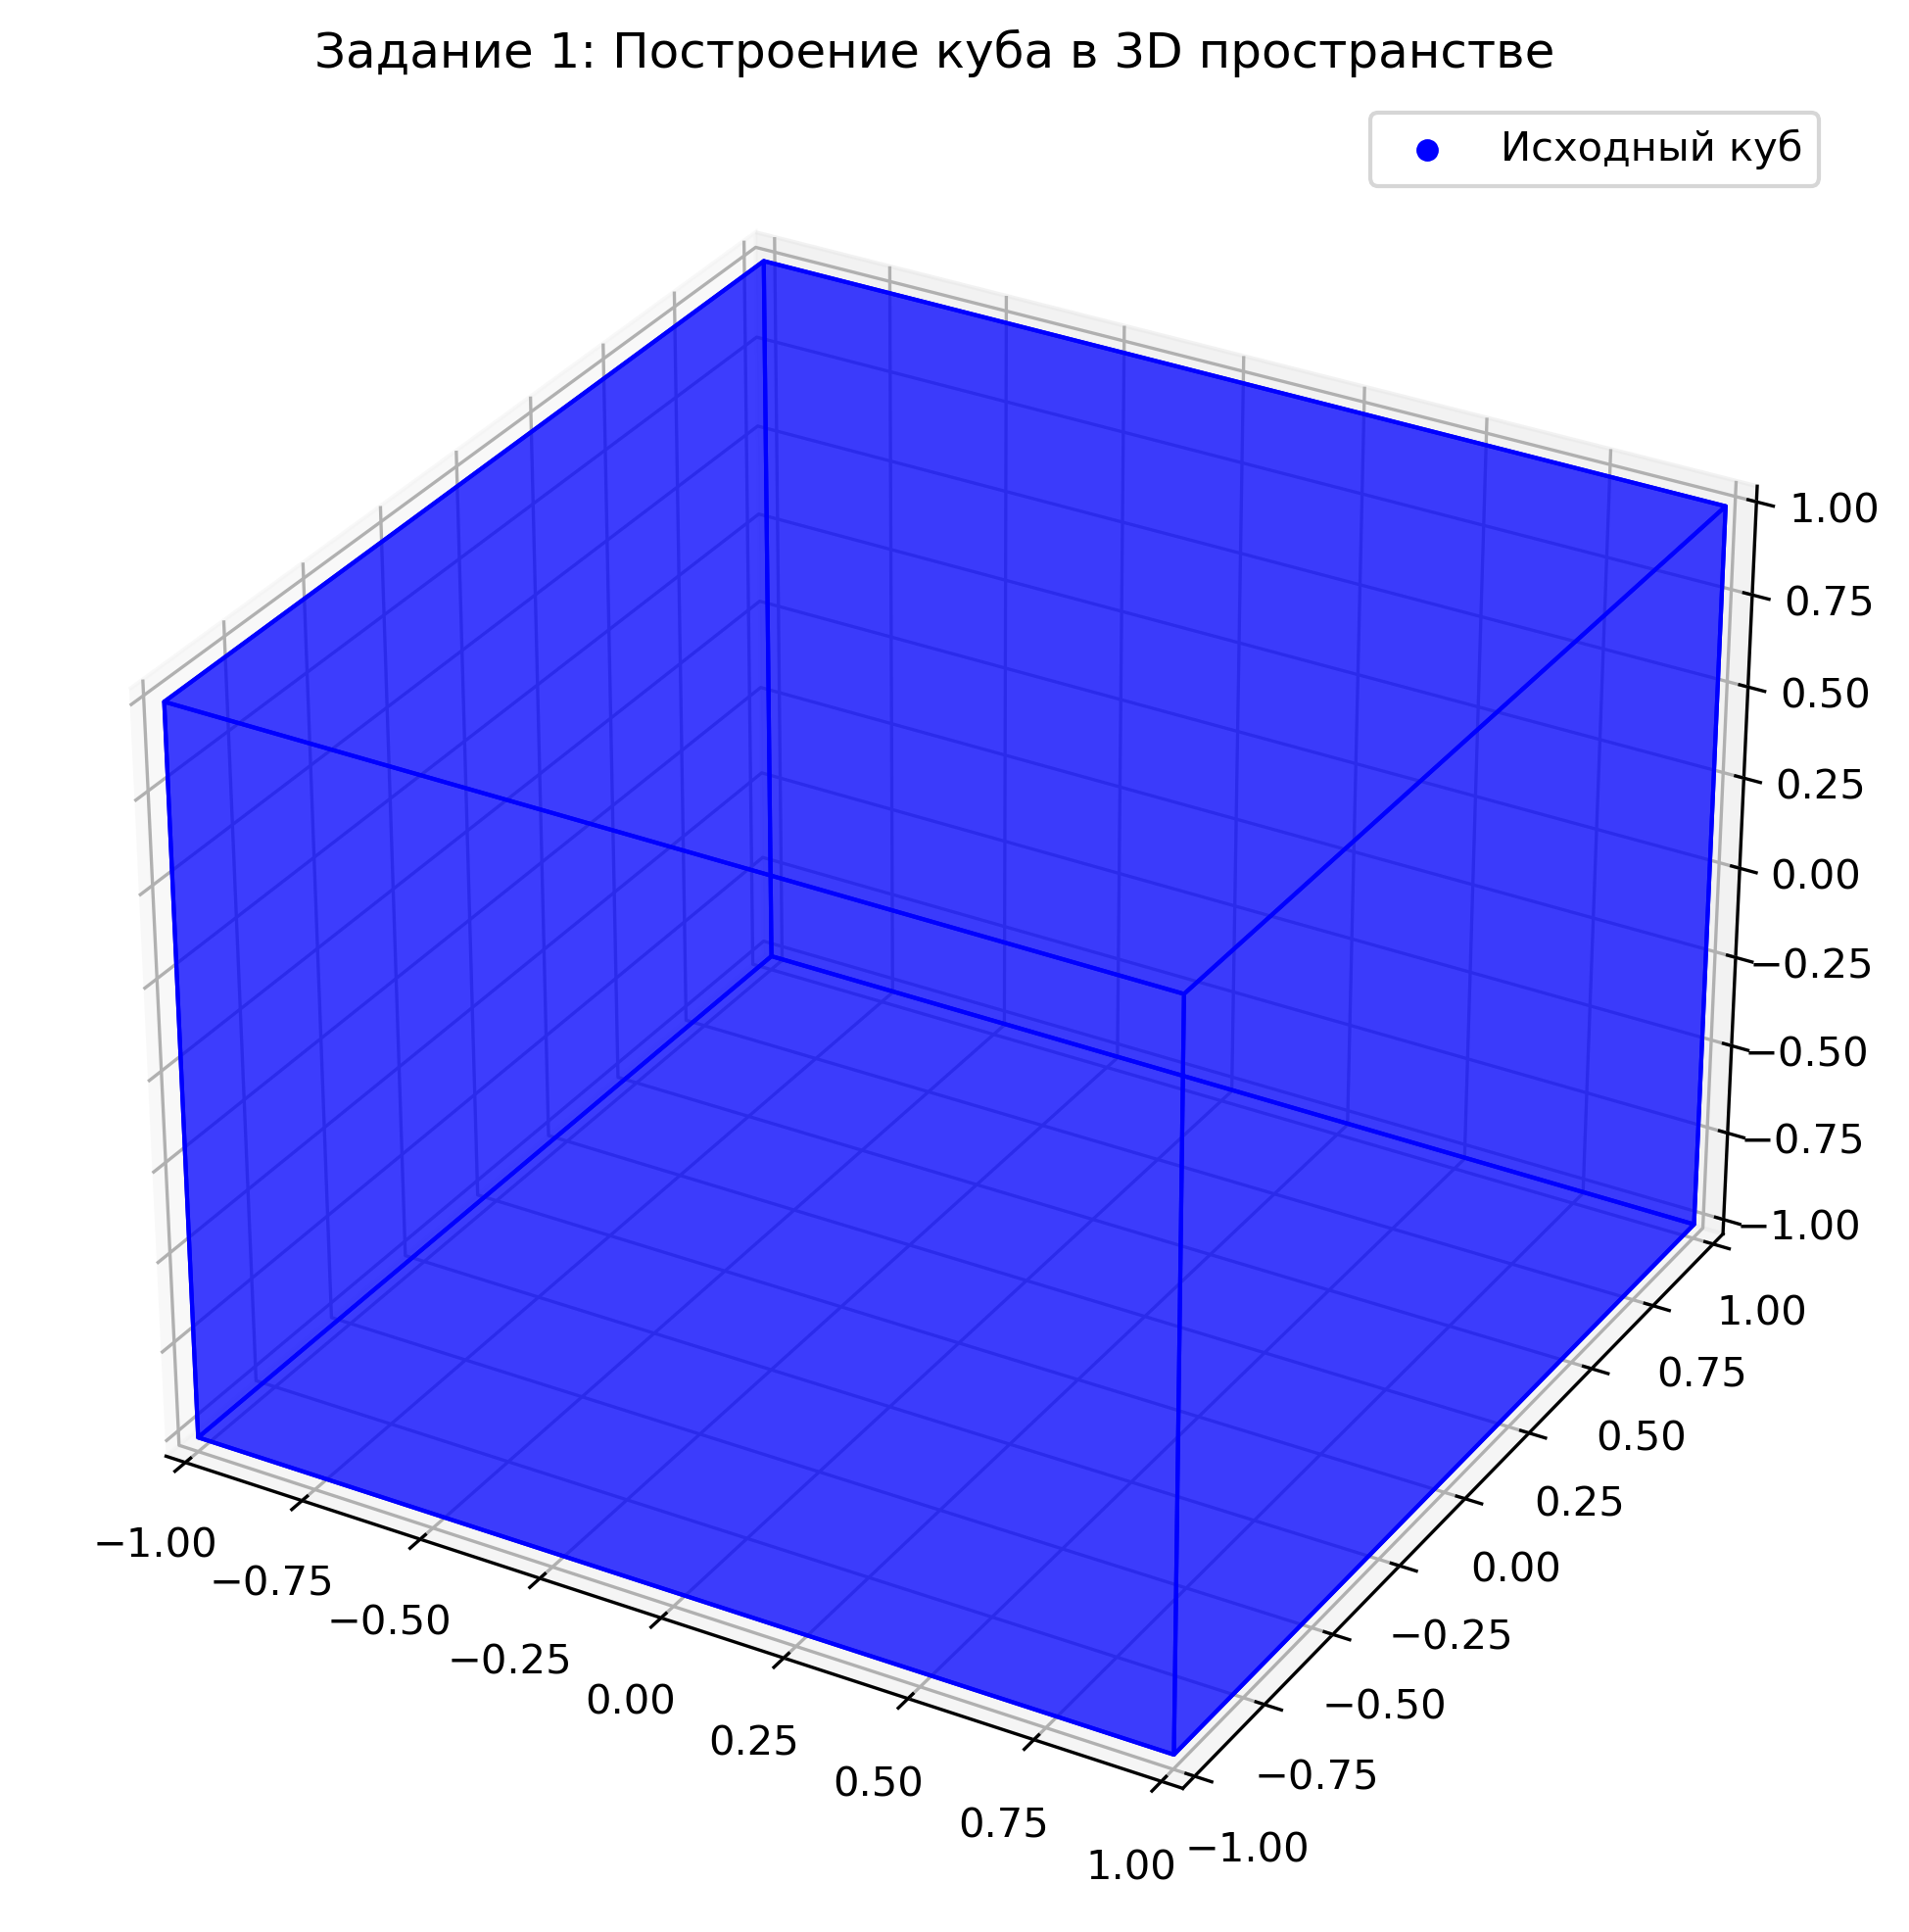
\includegraphics[width=0.5\textwidth]{task1/cube_original.png}
    \caption{Задание 1: Куб в трёхмерном пространстве}
\end{figure}

\begin{figure}[h!]
    \centering
    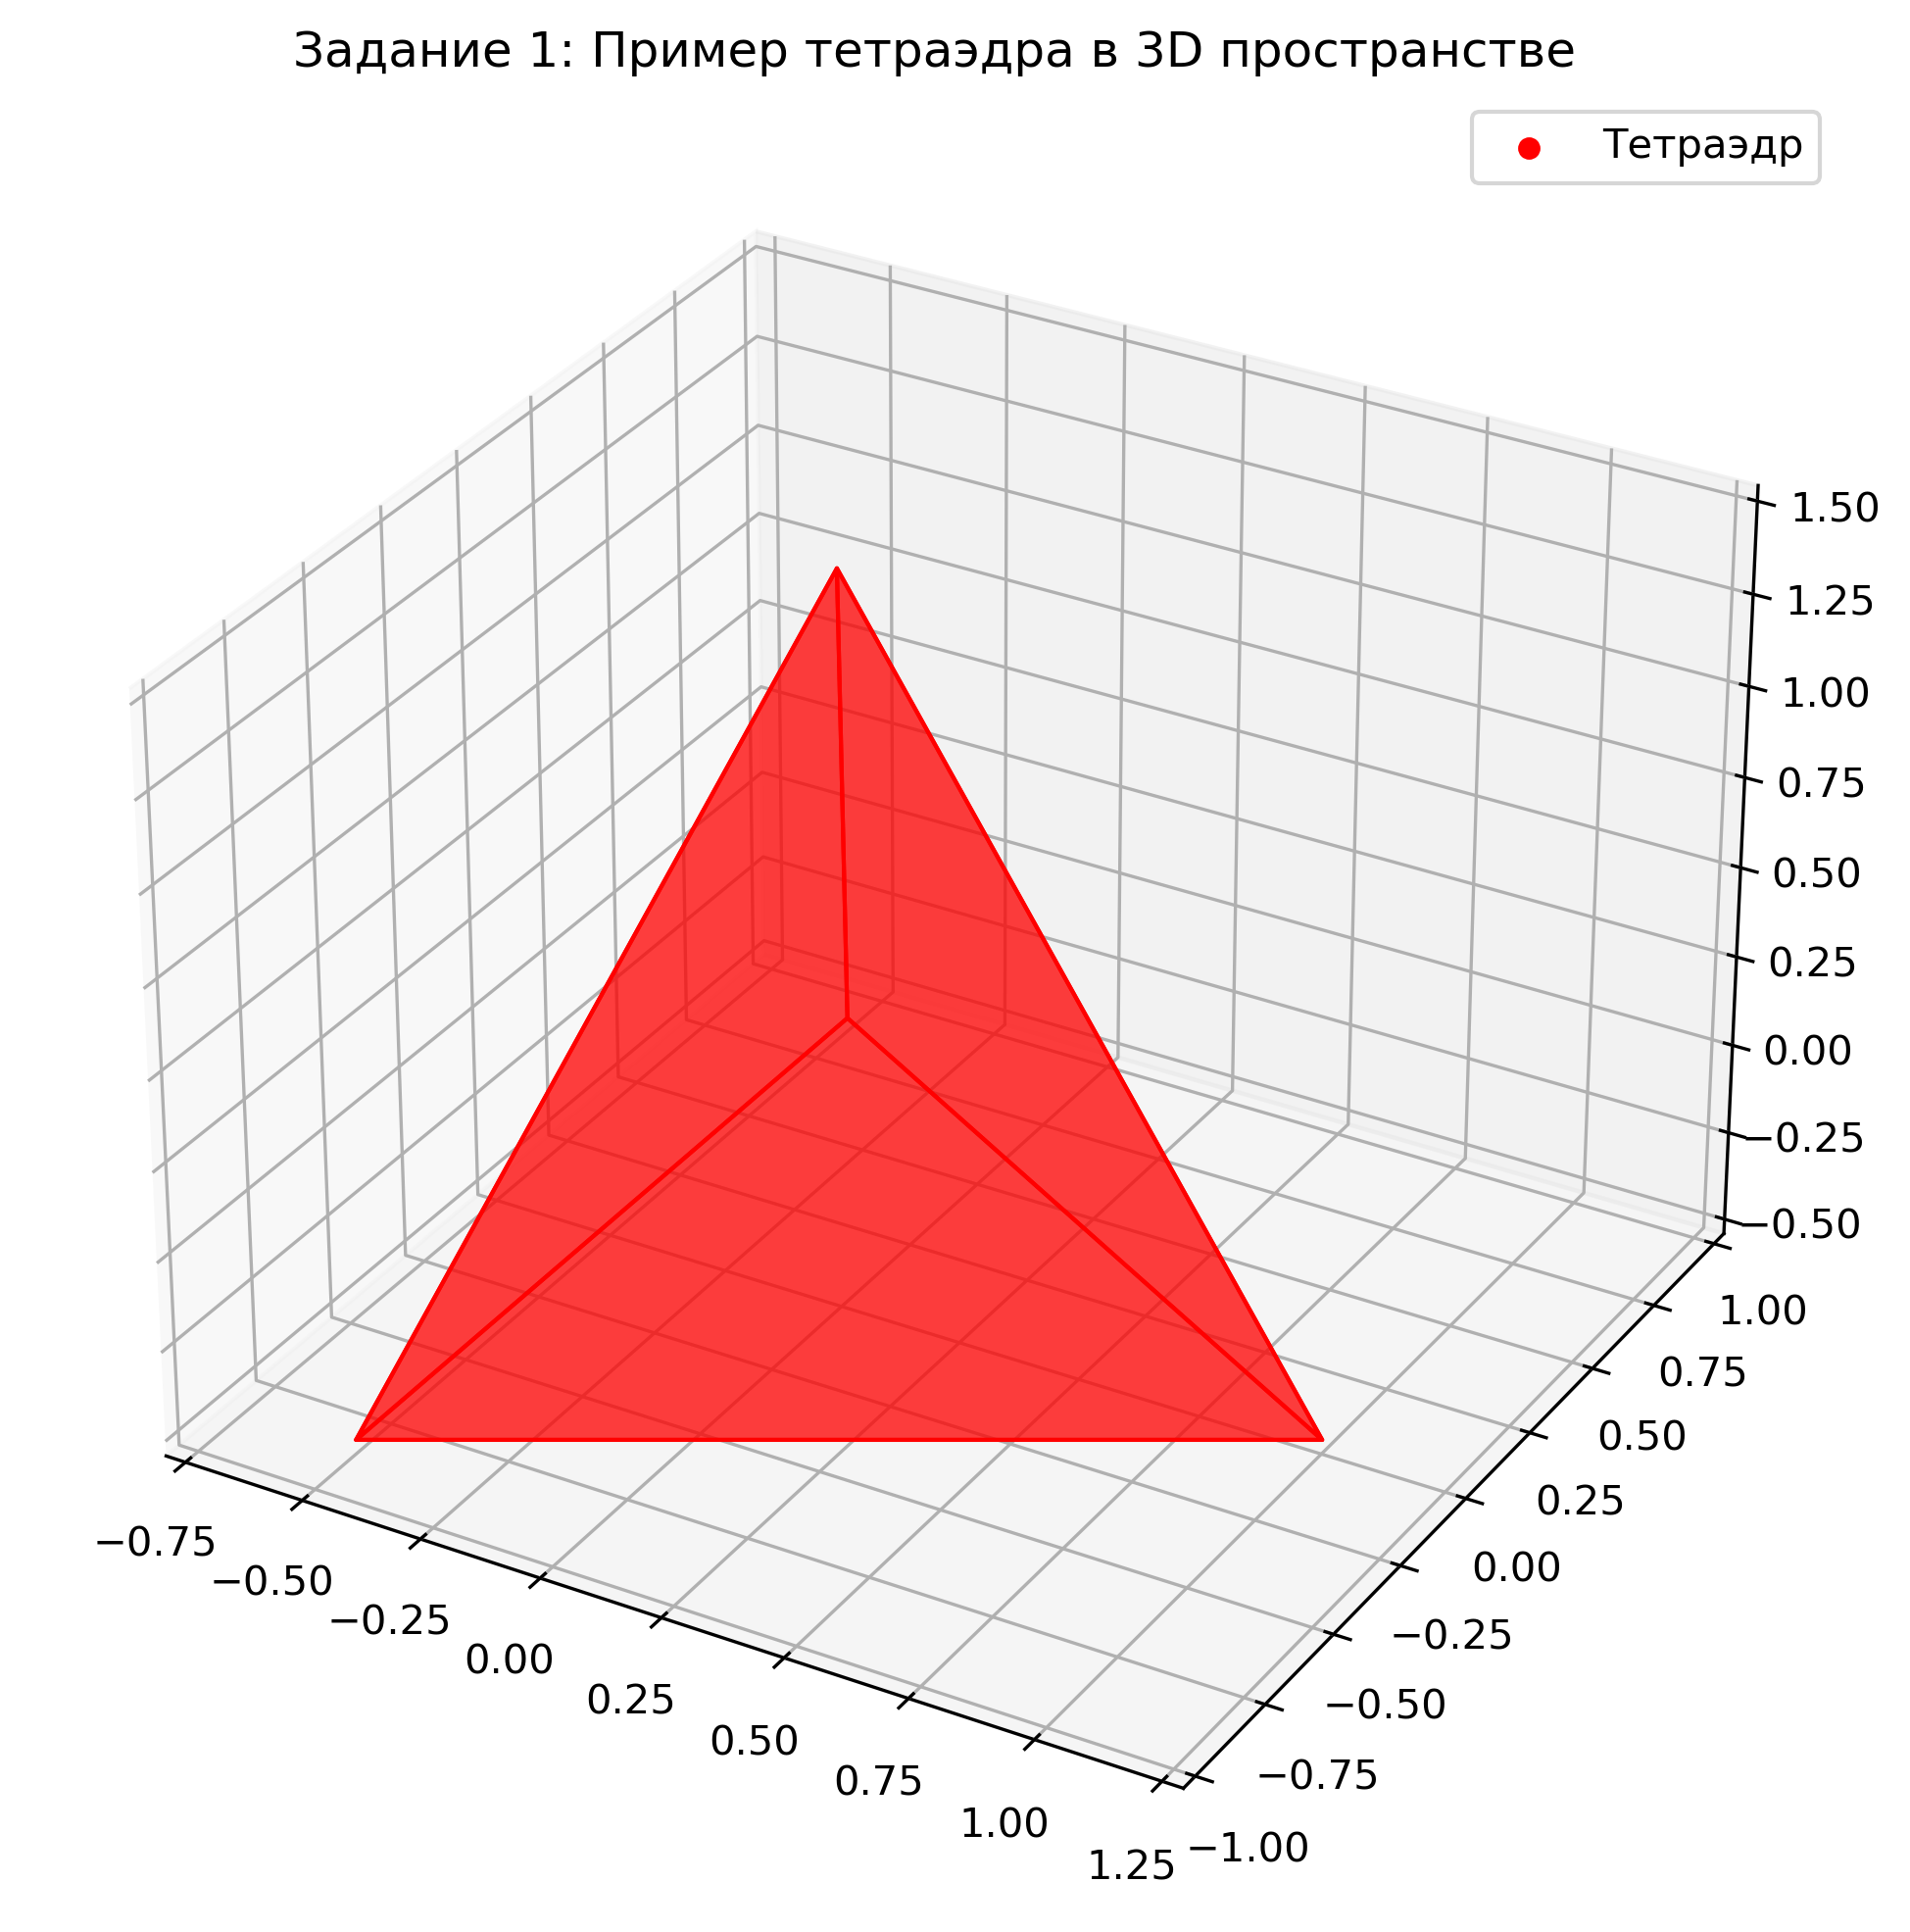
\includegraphics[width=0.5\textwidth]{task1/tetrahedron.png}
    \caption{Задание 1: Пример тетраэдра в трёхмерном пространстве}
\end{figure}

\section{Задание 2. Масштабирование куба}

Для изменения размеров куба используется матрица масштабирования:
\[
S = \begin{bmatrix}
    s_x & 0 & 0 & 0 \\
    0 & s_y & 0 & 0 \\
    0 & 0 & s_z & 0 \\
    0 & 0 & 0 & 1
\end{bmatrix}
\]
Здесь $s_x$, $s_y$, $s_z$ --- коэффициенты масштабирования по осям $X$, $Y$, $Z$ соответственно. Применяя $S$ к координатам вершин, получаем увеличенный или уменьшенный куб.

\begin{figure}[h!]
    \centering
    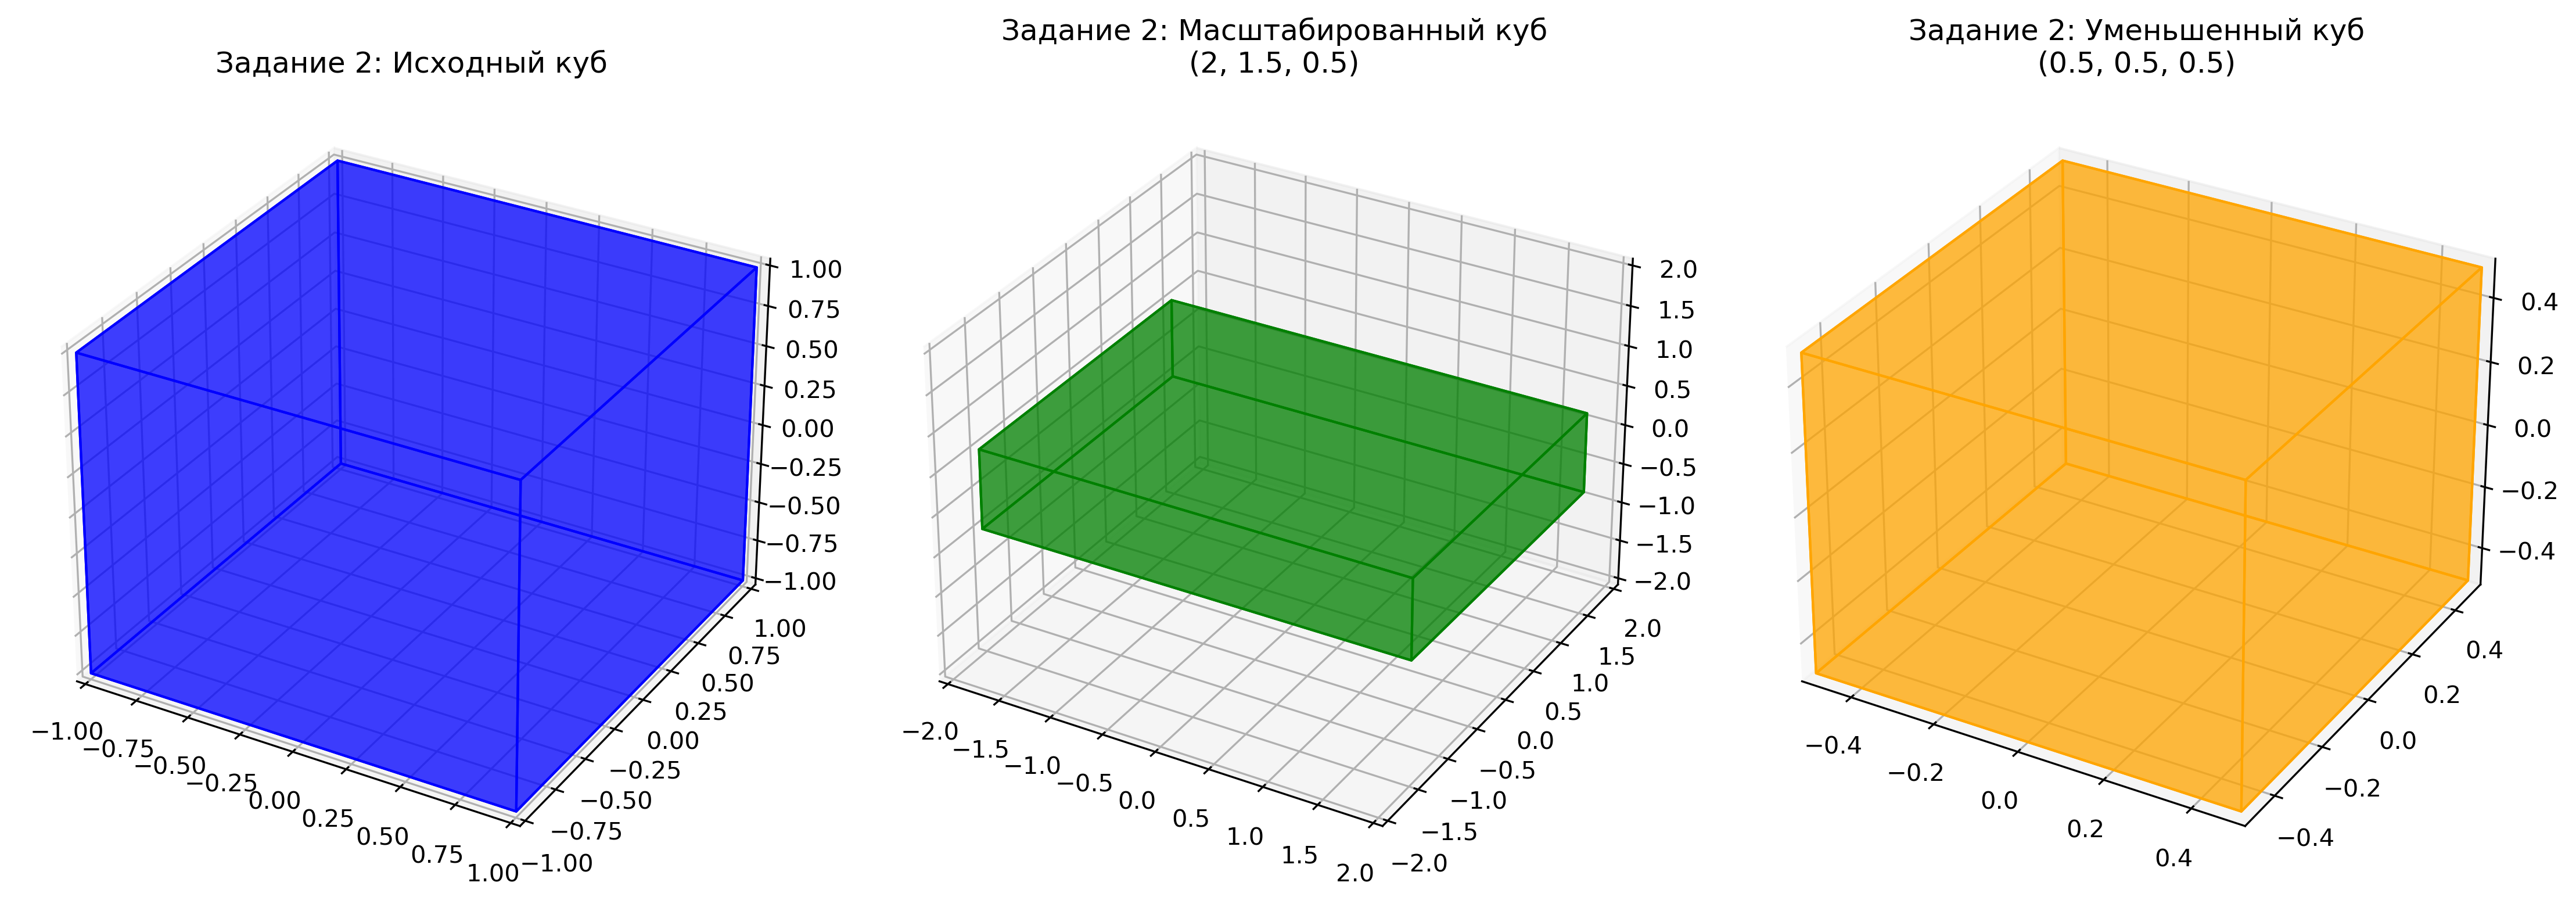
\includegraphics[width=\textwidth]{task2/scaling_comparison.png}
    \caption{Задание 2: Сравнение масштабирования куба: исходный, увеличенный (2, 1.5, 0.5) и уменьшенный (0.5, 0.5, 0.5)}
\end{figure}

\section{Задание 3. Перенос куба}

Для перемещения объекта в пространстве используется матрица сдвига:
\[
T = \begin{bmatrix}
    1 & 0 & 0 & t_x \\
    0 & 1 & 0 & t_y \\
    0 & 0 & 1 & t_z \\
    0 & 0 & 0 & 1
\end{bmatrix}
\]
Здесь $t_x$, $t_y$, $t_z$ --- величины смещения по соответствующим осям. Итоговые координаты получаются умножением $T$ на вектор вершин.

\begin{figure}[h!]
    \centering
    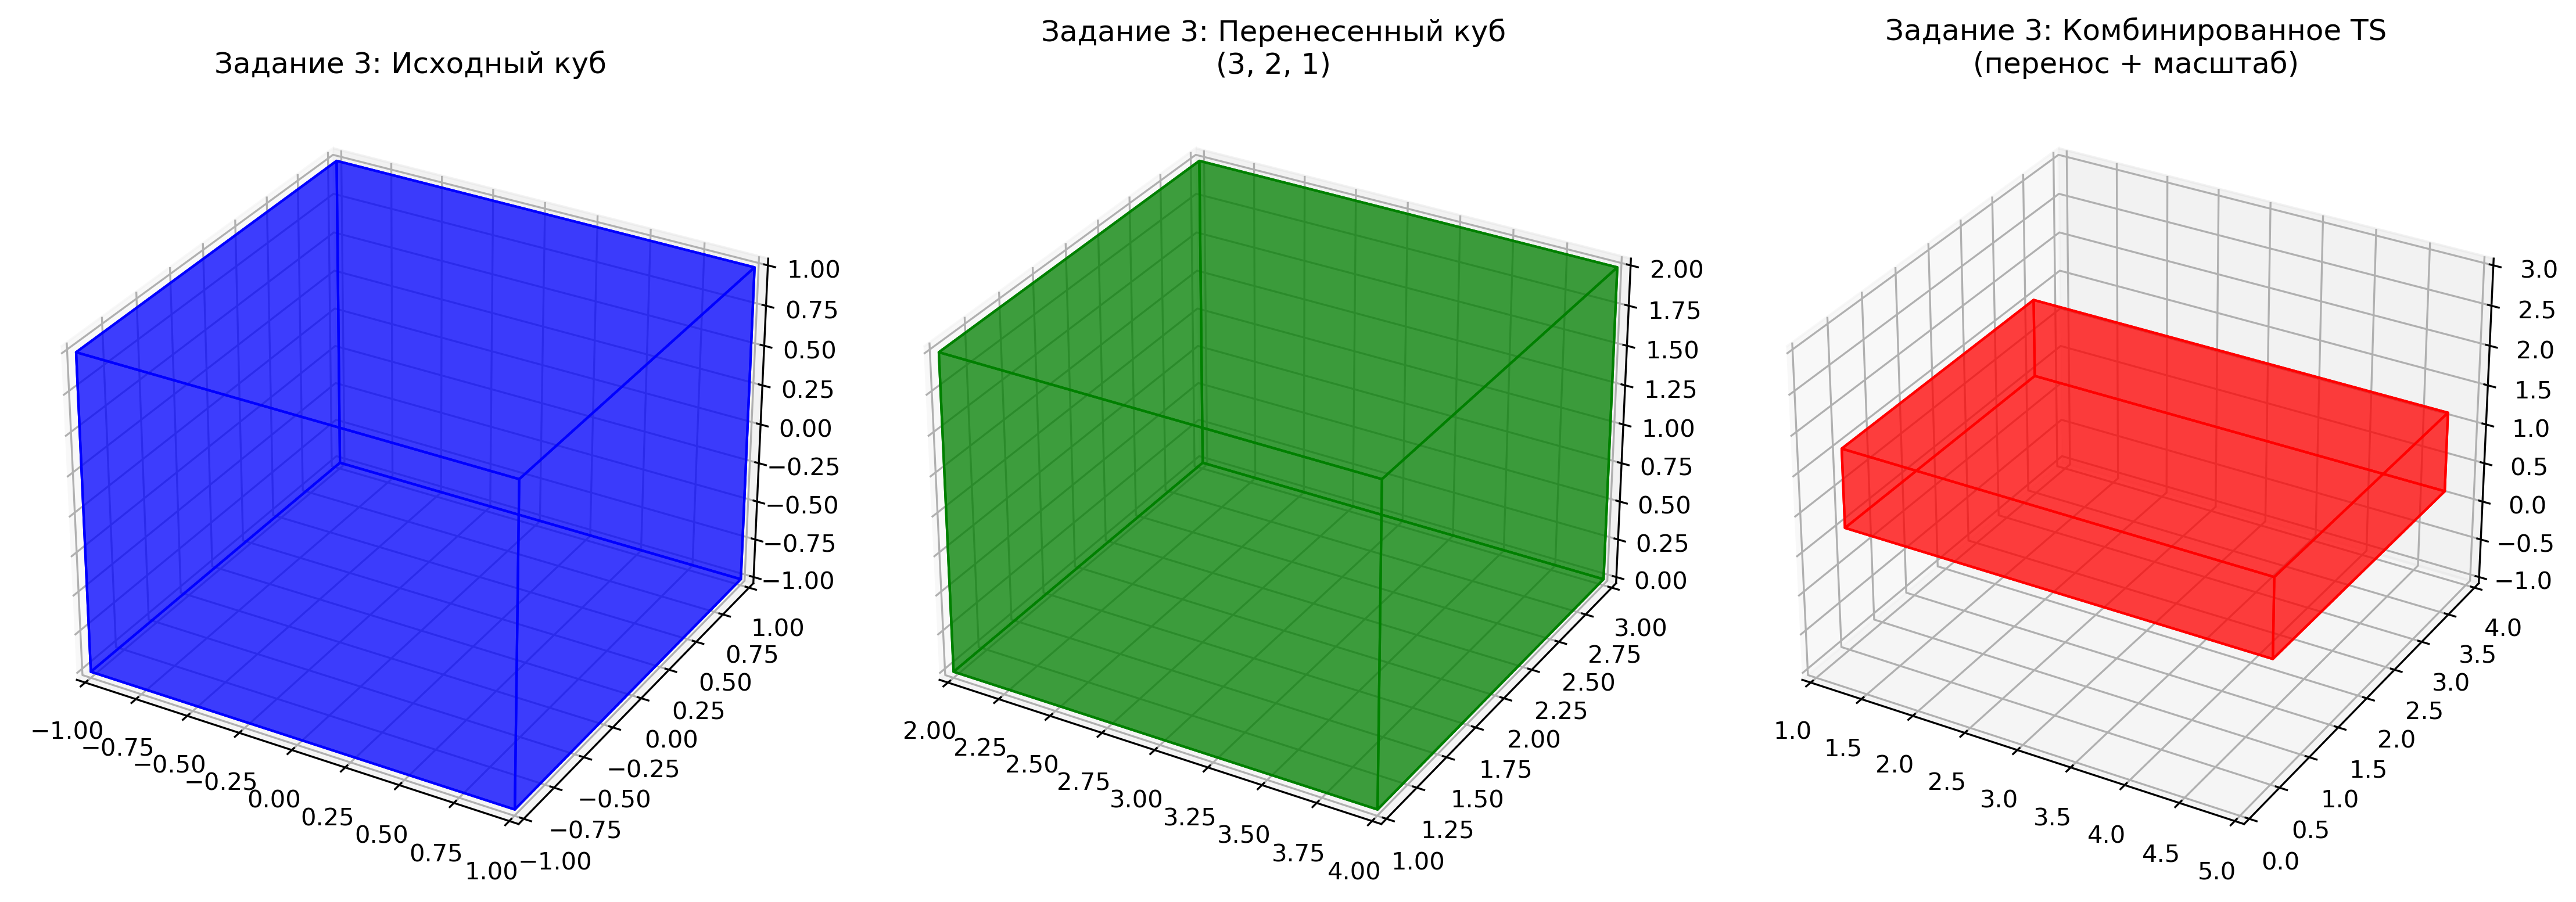
\includegraphics[width=\textwidth]{task3/translation_comparison.png}
    \caption{Задание 3: Сравнение переноса куба: исходный, перенесенный (3, 2, 1) и комбинированное преобразование TS}
\end{figure}

\textbf{Исследование коммутативности преобразований}

Важно отметить, что порядок применения матриц имеет значение. Рассмотрим композиции $TS$ (перенос, затем масштабирование) и $ST$ (масштабирование, затем перенос):

\begin{figure}[h!]
    \centering
    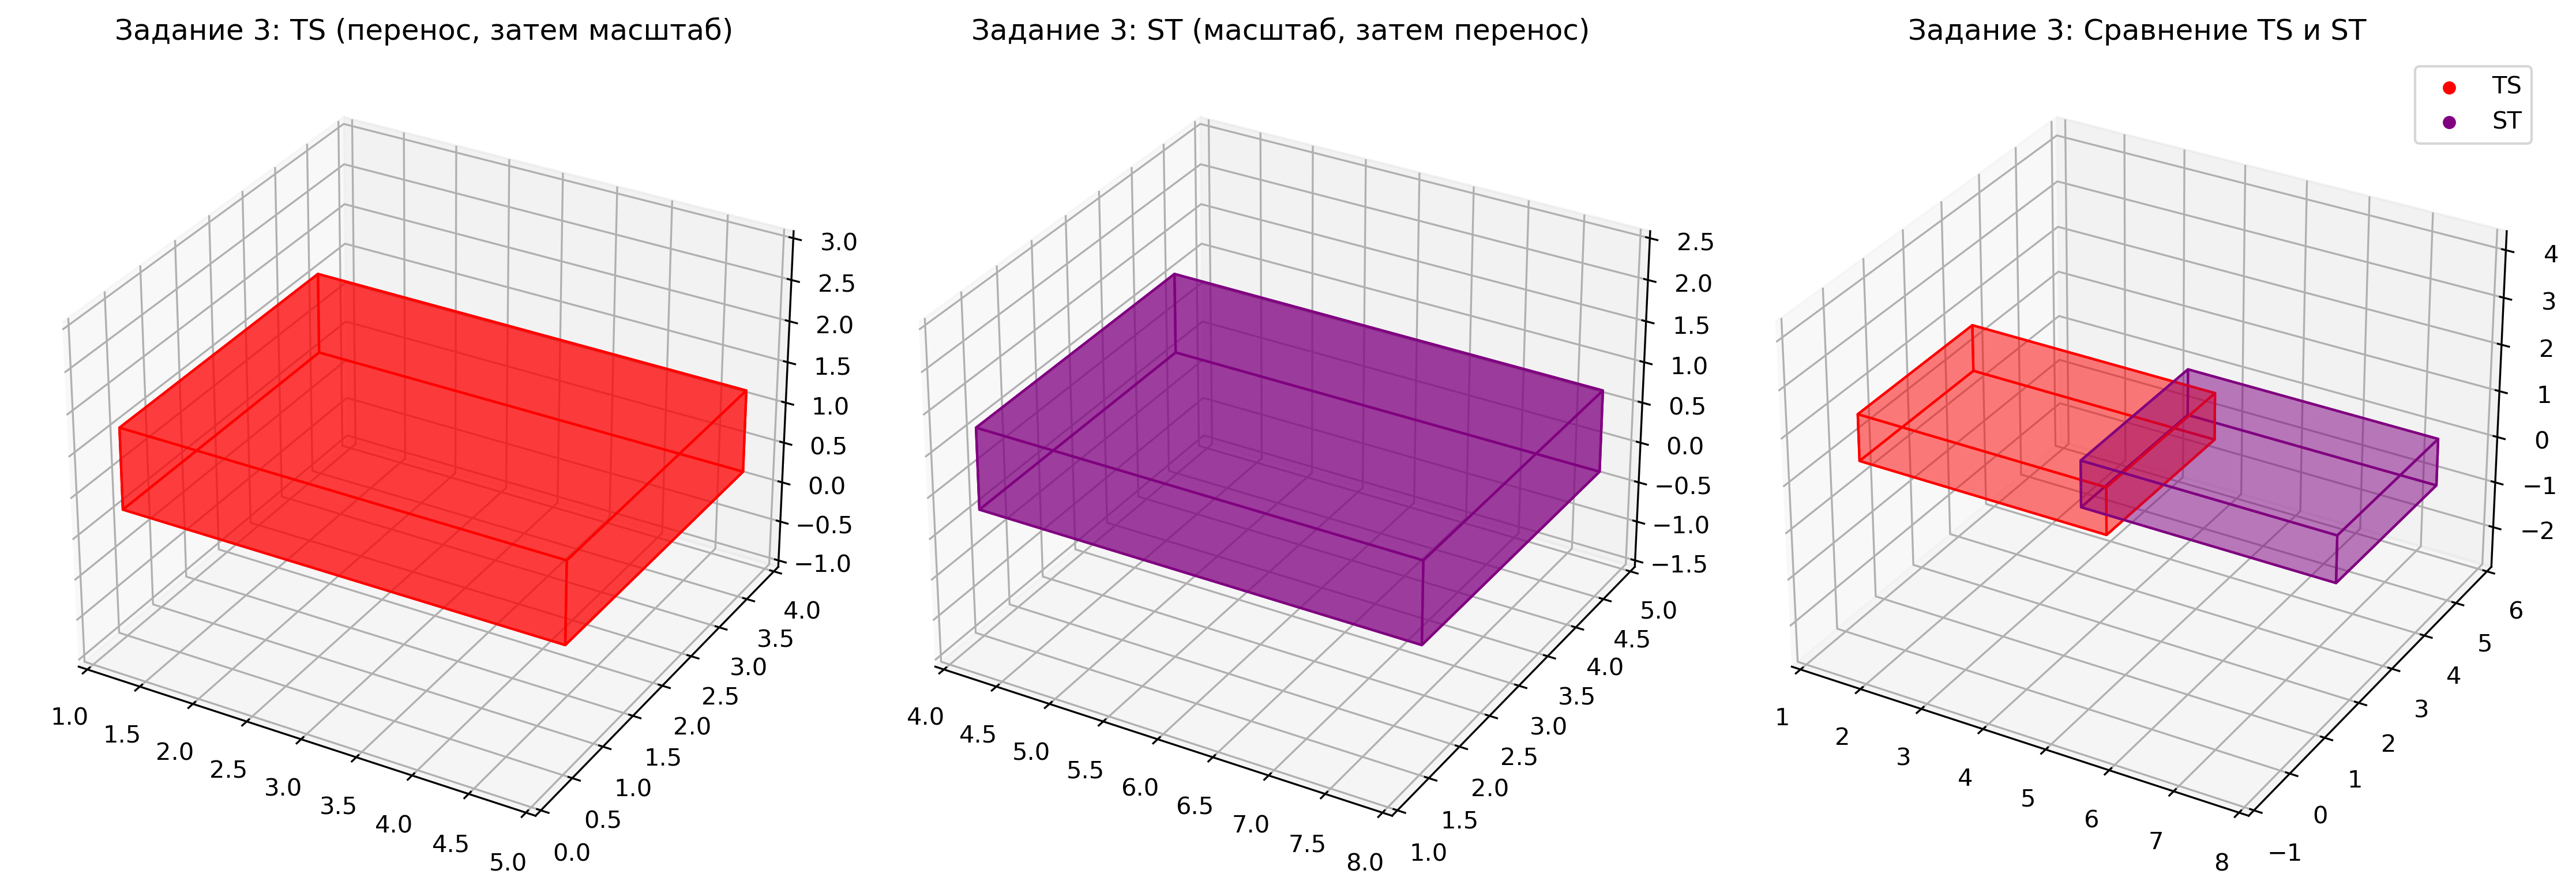
\includegraphics[width=\textwidth]{task3/ts_vs_st.png}
    \caption{Задание 3: Сравнение TS и ST: преобразования не коммутируют}
\end{figure}

Как видно из рисунка, $TS \neq ST$, что демонстрирует некоммутативность аффинных преобразований.

\section{Задание 4. Поворот куба}

Для поворота используются стандартные матрицы вращения вокруг осей:
\begin{itemize}
    \item \textbf{Вокруг $X$:}
    \[
    R_x(\theta) = \begin{bmatrix}
        1 & 0 & 0 & 0 \\
        0 & \cos\theta & -\sin\theta & 0 \\
        0 & \sin\theta & \cos\theta & 0 \\
        0 & 0 & 0 & 1
    \end{bmatrix}
    \]
    \item \textbf{Вокруг $Y$:}
    \[
    R_y(\theta) = \begin{bmatrix}
        \cos\theta & 0 & \sin\theta & 0 \\
        0 & 1 & 0 & 0 \\
        -\sin\theta & 0 & \cos\theta & 0 \\
        0 & 0 & 0 & 1
    \end{bmatrix}
    \]
    \item \textbf{Вокруг $Z$:}
    \[
    R_z(\theta) = \begin{bmatrix}
        \cos\theta & -\sin\theta & 0 & 0 \\
        \sin\theta & \cos\theta & 0 & 0 \\
        0 & 0 & 1 & 0 \\
        0 & 0 & 0 & 1
    \end{bmatrix}
    \]
\end{itemize}

\textbf{Поворот вокруг произвольной оси}

Для поворота вокруг произвольной оси $v$ на угол $\theta$ используется формула Родрига:
\[
v = \begin{bmatrix} v_x \\ v_y \\ v_z \end{bmatrix}, \quad J = \frac{1}{\|v\|} \begin{bmatrix}
0 & -v_z & v_y & 0 \\
v_z & 0 & -v_x & 0 \\
-v_y & v_x & 0 & 0 \\
0 & 0 & 0 & 0
\end{bmatrix}, \quad R_v(\theta) = e^{J\theta}
\]

\begin{figure}[h!]
    \centering
    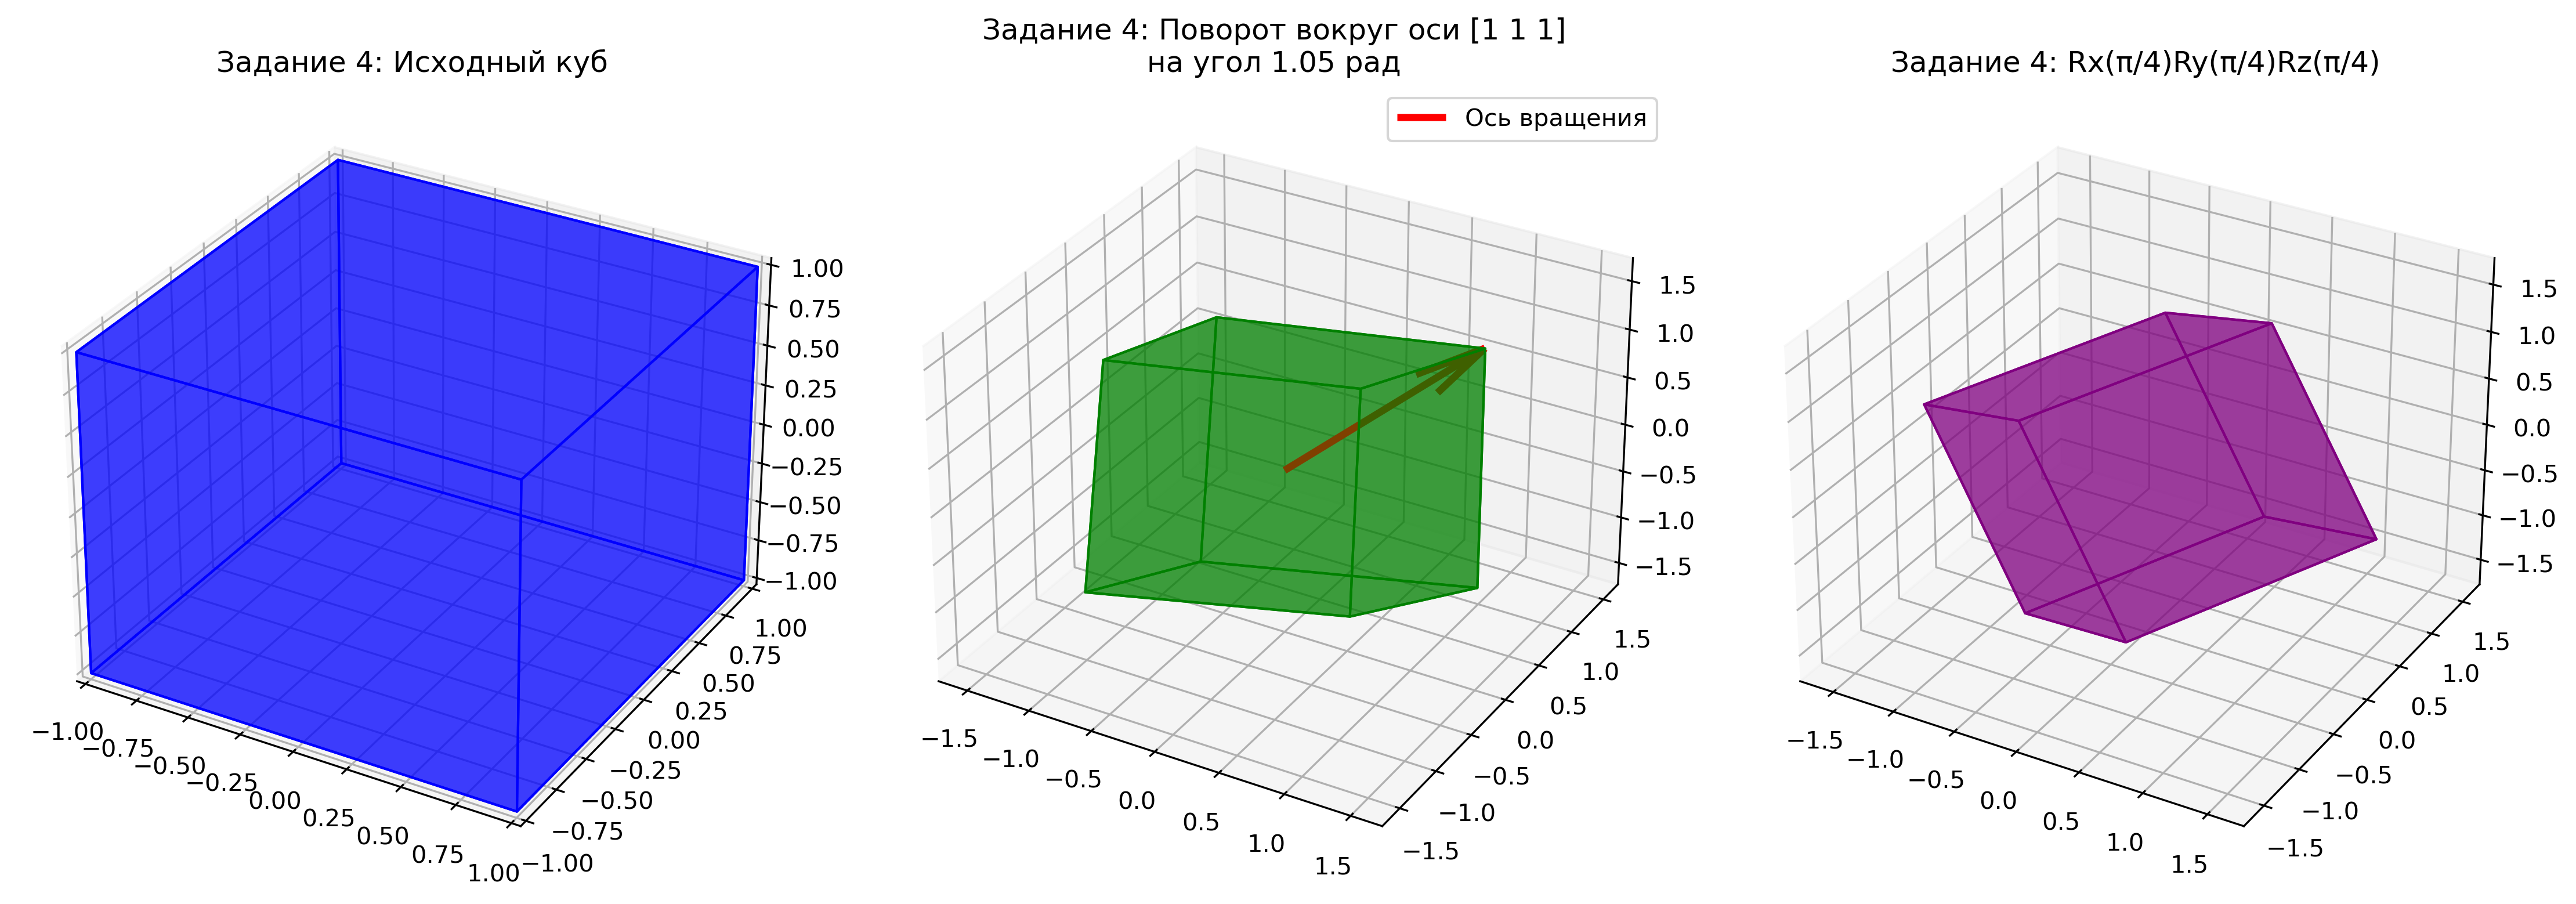
\includegraphics[width=\textwidth]{task4/rotation_analysis.png}
    \caption{Задание 4: Анализ поворотов: исходный куб, поворот вокруг произвольной оси (1,1,1) и композиция поворотов вокруг координатных осей}
\end{figure}

\textbf{Ответы на вопросы задания:}
\begin{itemize}
    \item Матрицы $R_x(\theta)$, $R_y(\phi)$, $R_z(\psi)$ получаются при выборе вектора $v$ вдоль осей $x$, $y$ или $z$ соответственно.
    \item Тройка матриц $R_x(\theta)R_y(\phi)R_z(\psi)$ достаточна для описания всех возможных вращений в 3D пространстве (теорема Эйлера).
    \item Ось вращения можно восстановить, найдя собственный вектор матрицы поворота, соответствующий собственному значению 1.
\end{itemize}

\section{Задание 5. Поворот куба вокруг вершины}

Чтобы повернуть куб относительно одной из его вершин, нужно найти матрицу преобразования, которая осуществит поворот таким образом, что центр вращения будет совпадать с одной из его вершин.

\textbf{Найдем матрицу преобразования:}

Пусть $P$ --- координаты вершины, вокруг которой происходит поворот, $R$ --- матрица поворота вокруг оси, проходящей через начало координат. Тогда искомая матрица имеет вид:

\[
M = T \cdot R \cdot T^{-1}
\]

где $T$ --- матрица переноса, перемещающая вершину $P$ в начало координат:
\[
T = \begin{bmatrix}
1 & 0 & 0 & -P_x \\
0 & 1 & 0 & -P_y \\
0 & 0 & 1 & -P_z \\
0 & 0 & 0 & 1
\end{bmatrix}
\]

$T^{-1}$ --- обратная матрица переноса:
\[
T^{-1} = \begin{bmatrix}
1 & 0 & 0 & P_x \\
0 & 1 & 0 & P_y \\
0 & 0 & 1 & P_z \\
0 & 0 & 0 & 1
\end{bmatrix}
\]

\begin{figure}[h!]
    \centering
    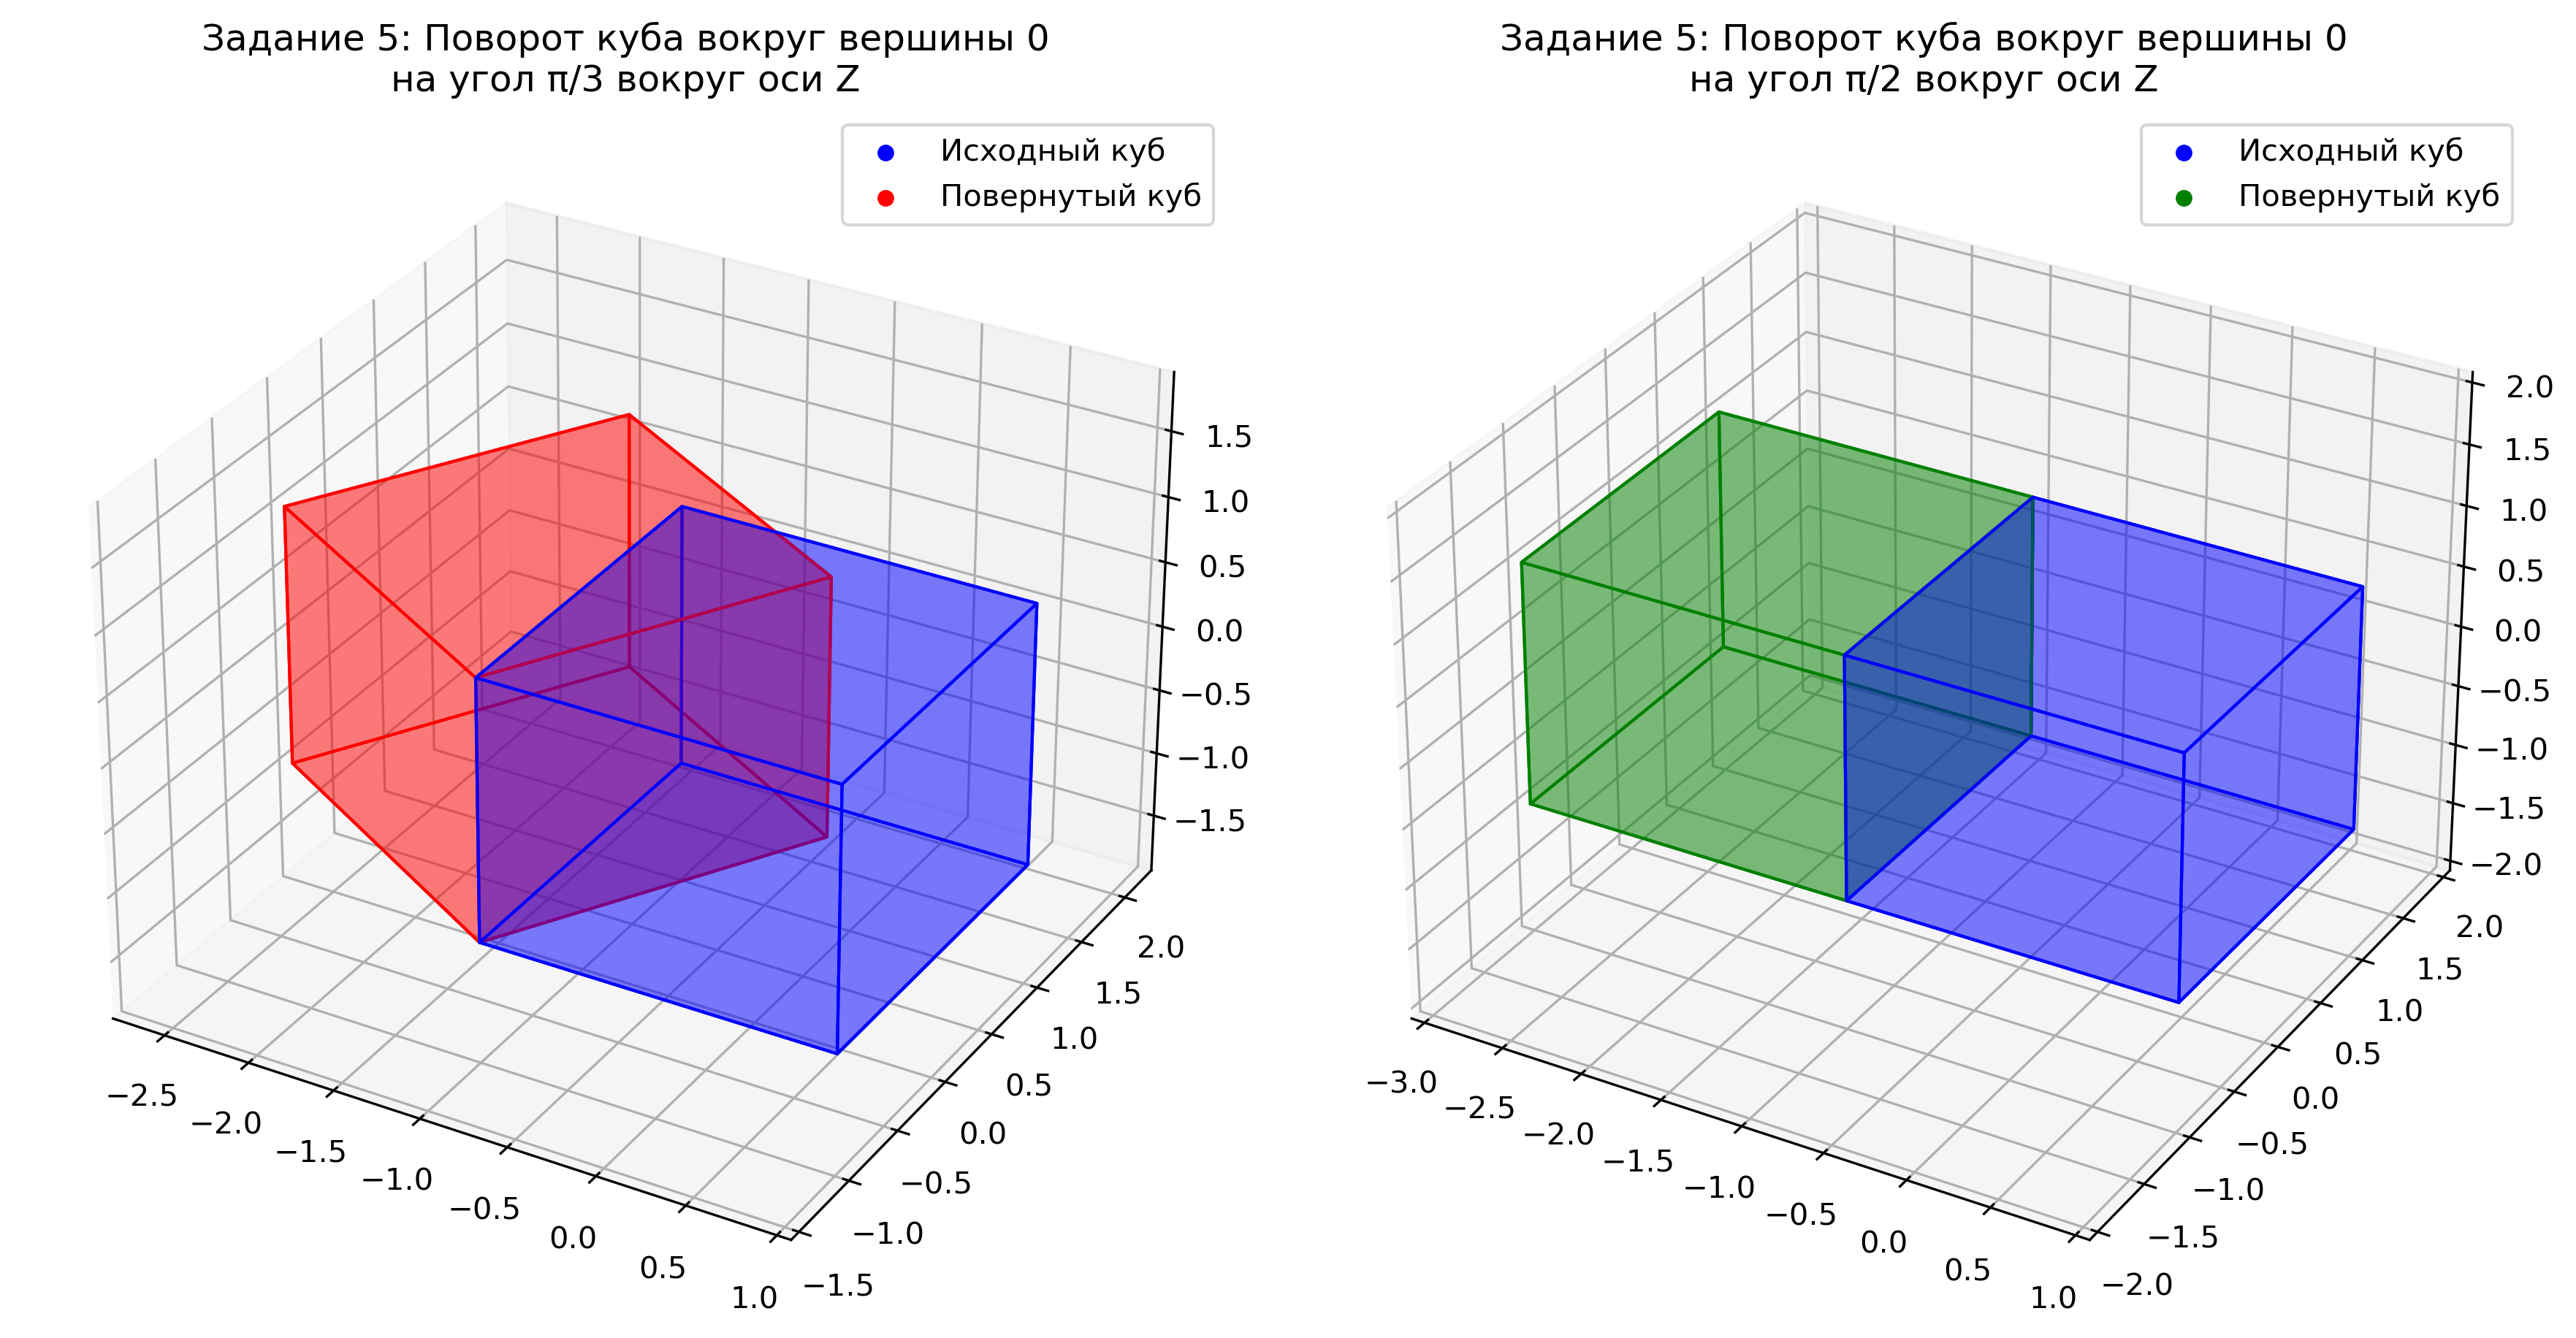
\includegraphics[width=\textwidth]{task5/rotation_around_vertex.png}
    \caption{Задание 5: Поворот куба вокруг вершины 0: на угол $\pi/3$ (слева) и $\pi/2$ (справа) вокруг оси Z}
\end{figure}

\section{Задание 6. Виртуальная камера}

Для имитации движения камеры сцены используются матрицы вращения и матрица переноса камеры:
\[
T_{camera} = \begin{bmatrix}
1 & 0 & 0 & -t_x \\
0 & 1 & 0 & -t_y \\
0 & 0 & 1 & -t_z \\
0 & 0 & 0 & 1
\end{bmatrix}
\]
Здесь $t_x$, $t_y$, $t_z$ --- положение камеры. Отрицательный знак означает, что движение камеры в одну сторону эквивалентно движению сцены в противоположную.

\begin{figure}[h!]
    \centering
    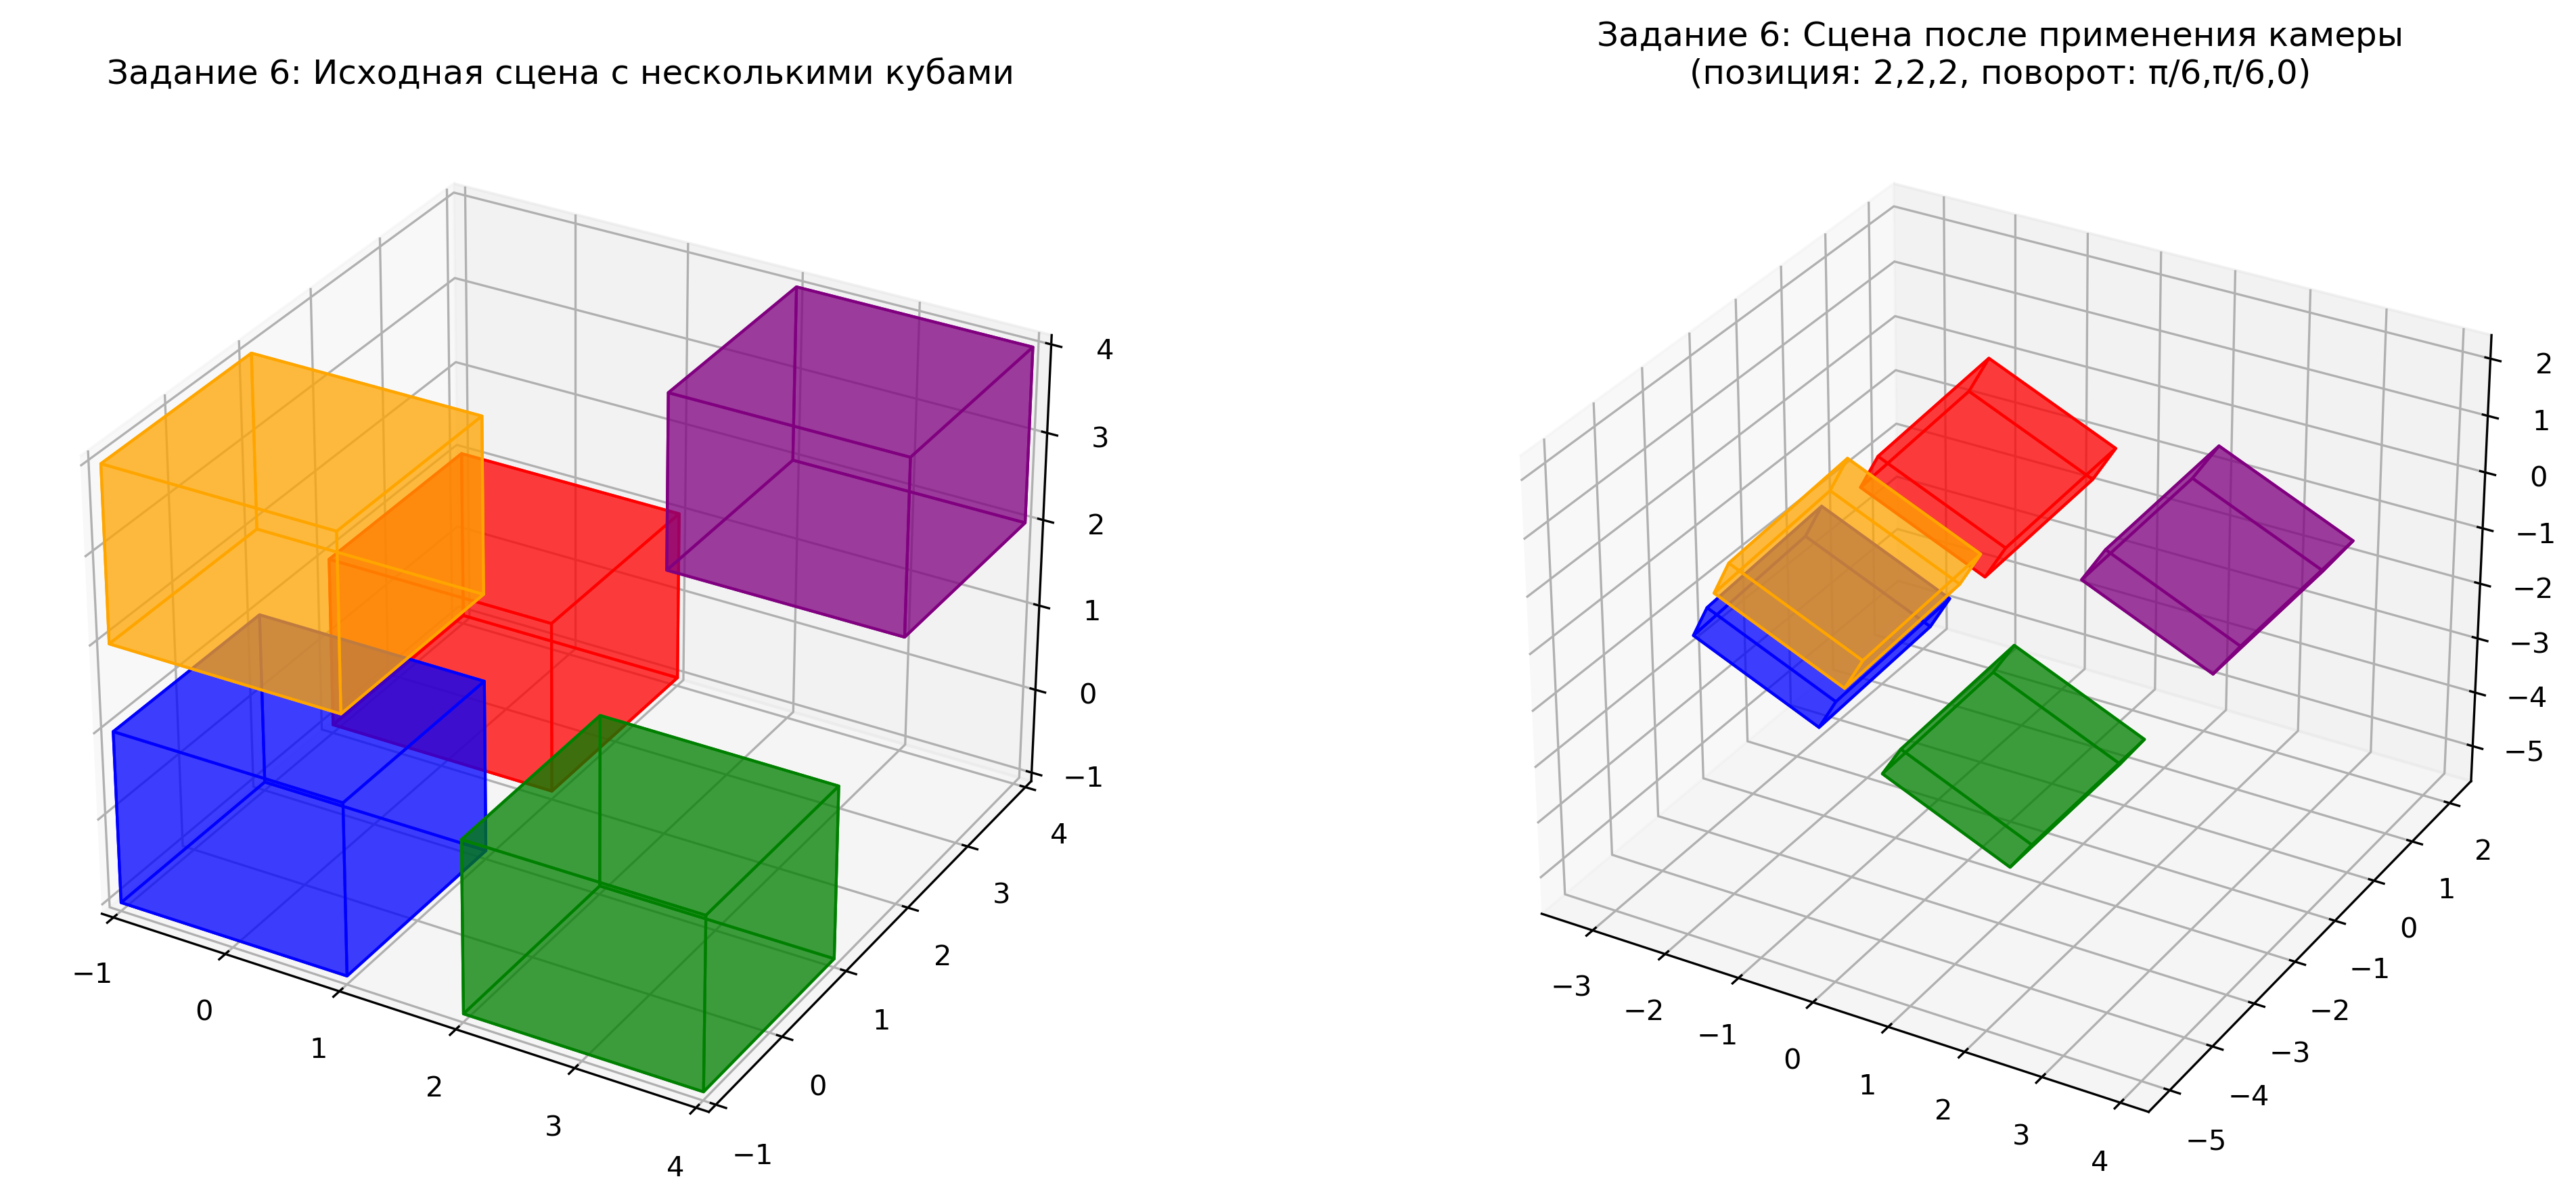
\includegraphics[width=\textwidth]{task6/camera_scene.png}
    \caption{Задание 6: Сцена с несколькими кубами: исходная (слева) и после применения камеры (справа)}
\end{figure}

Обратная матрица позволяет вернуть камеру в исходное положение.

\section{Задание 7. Перспективное отображение}

Для создания эффекта перспективы используется специальная матрица проекции:
\[
M_{proj} = \begin{bmatrix}
s & 0 & 0 & 0 \\
0 & s & 0 & 0 \\
0 & 0 & \frac{f+ n}{f-n} & -1 \\
0 & 0 & \frac{2fn}{f-n} & 0
\end{bmatrix}
\]
Параметры:
\begin{itemize}
    \item $s = \frac{1}{\tan(\frac{\text{fov}}{2})}$ --- масштаб по $X$ и $Y$ (fov --- угол обзора).
    \item $f$, $n$ --- дальняя и ближняя плоскости отсечения.
    \item Остальные элементы отвечают за нормализацию глубины и перспективу.
\end{itemize}

\begin{figure}[h!]
    \centering
    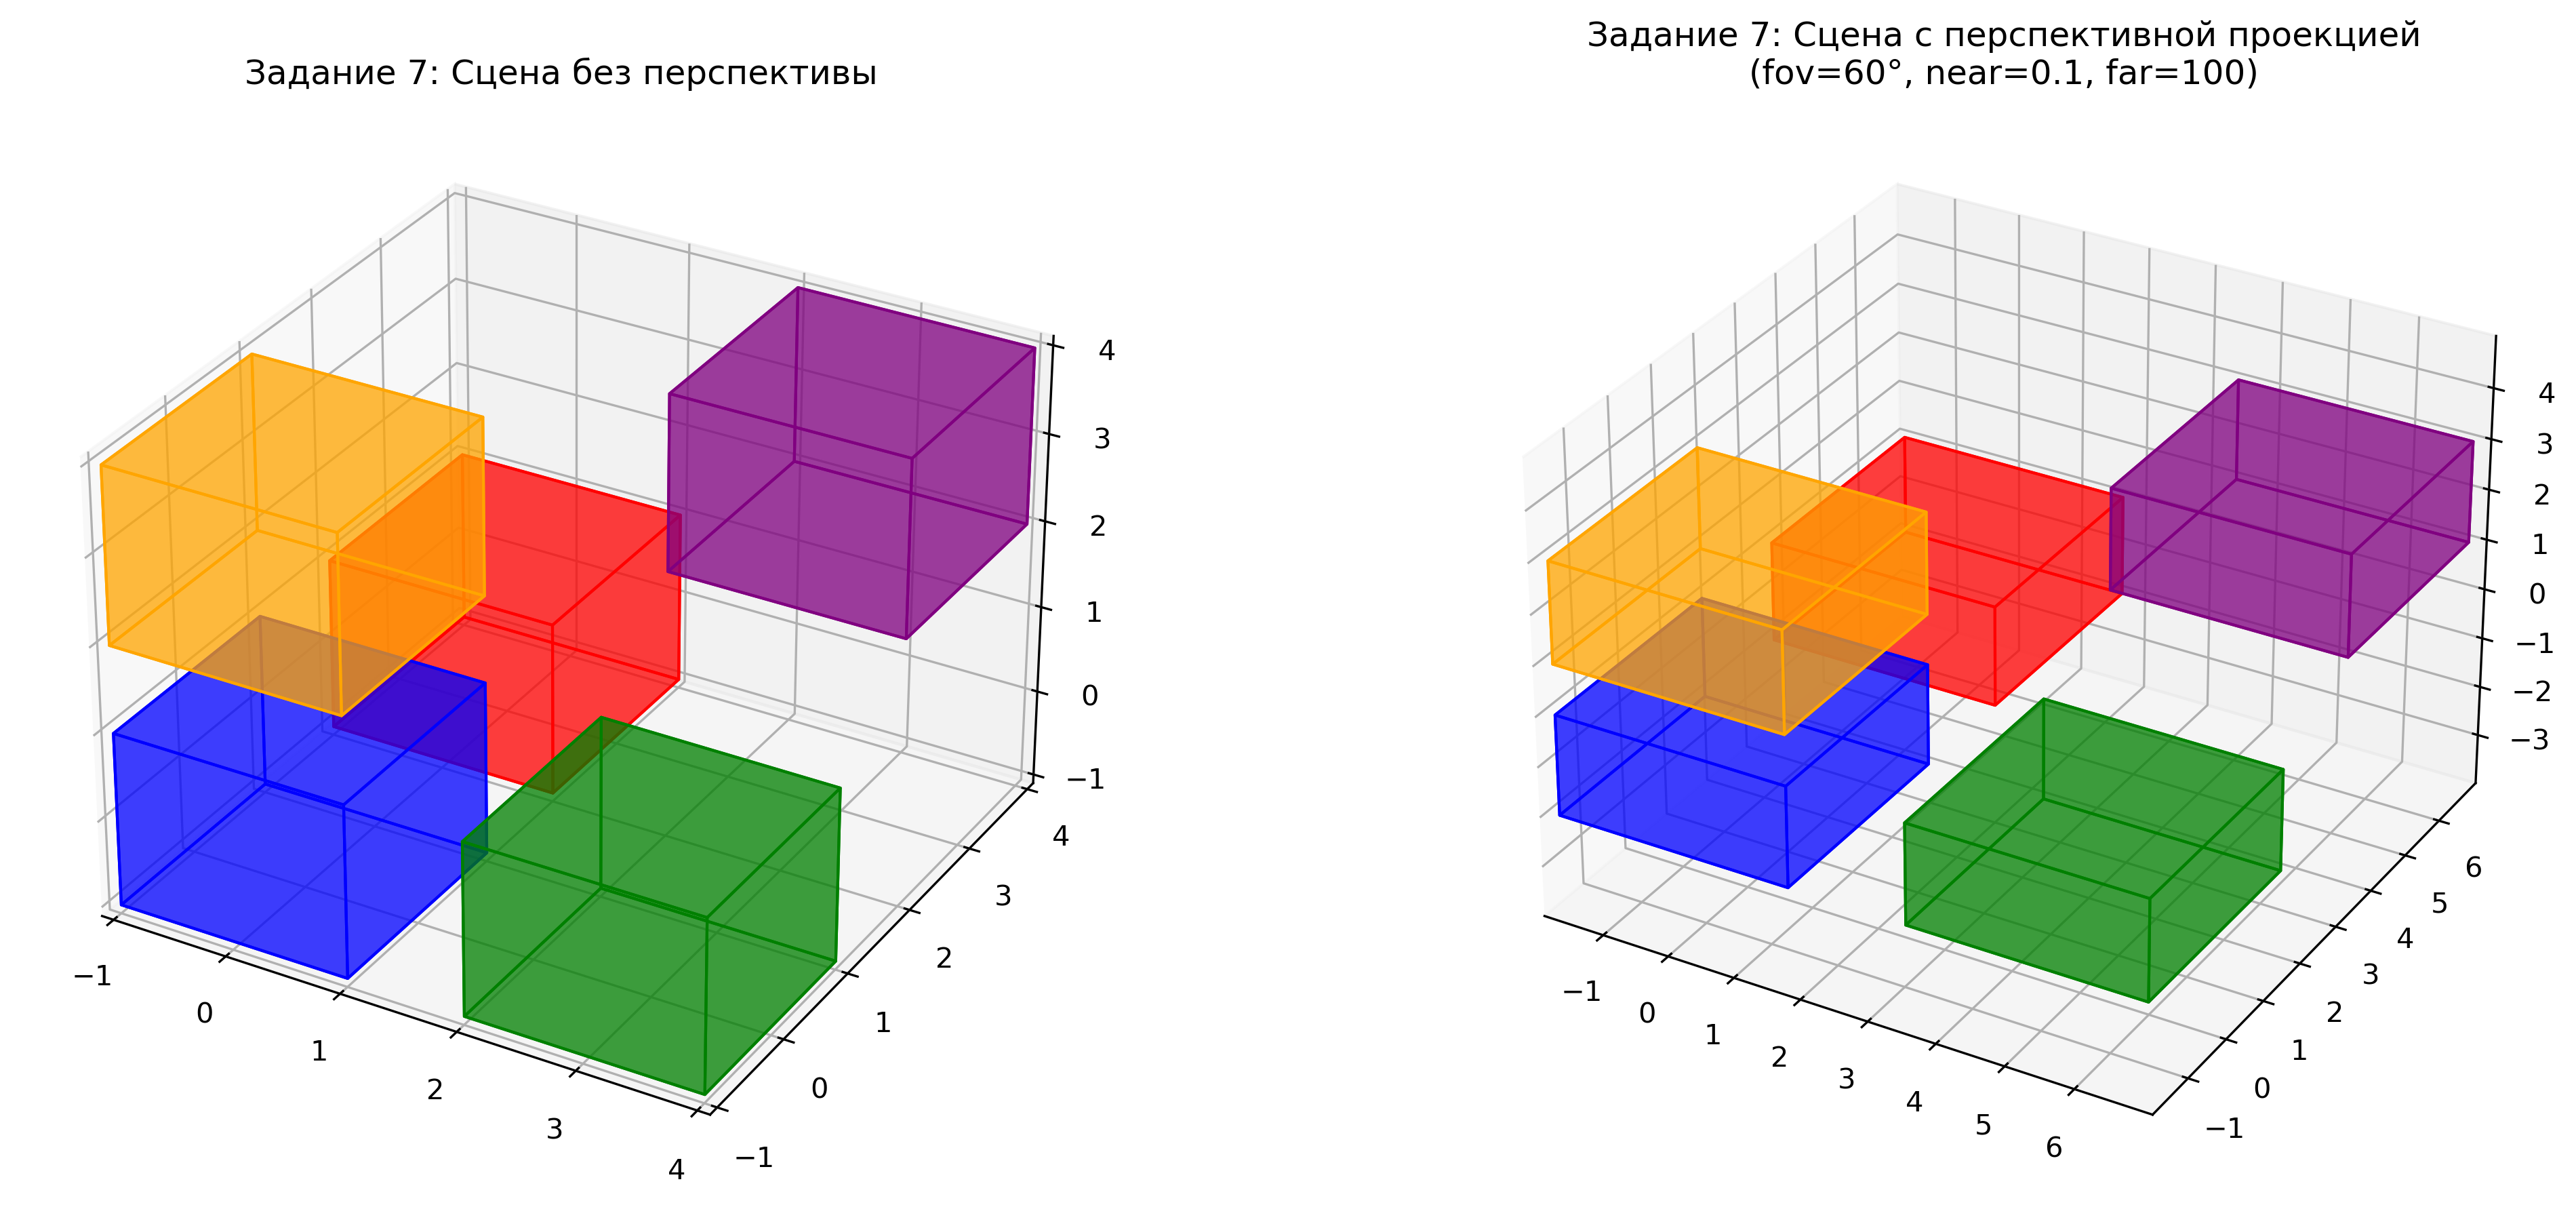
\includegraphics[width=\textwidth]{task7/perspective_comparison.png}
    \caption{Задание 7: Сравнение сцены без перспективы (слева) и с перспективной проекцией (справа)}
\end{figure}

\begin{figure}[h!]
    \centering
    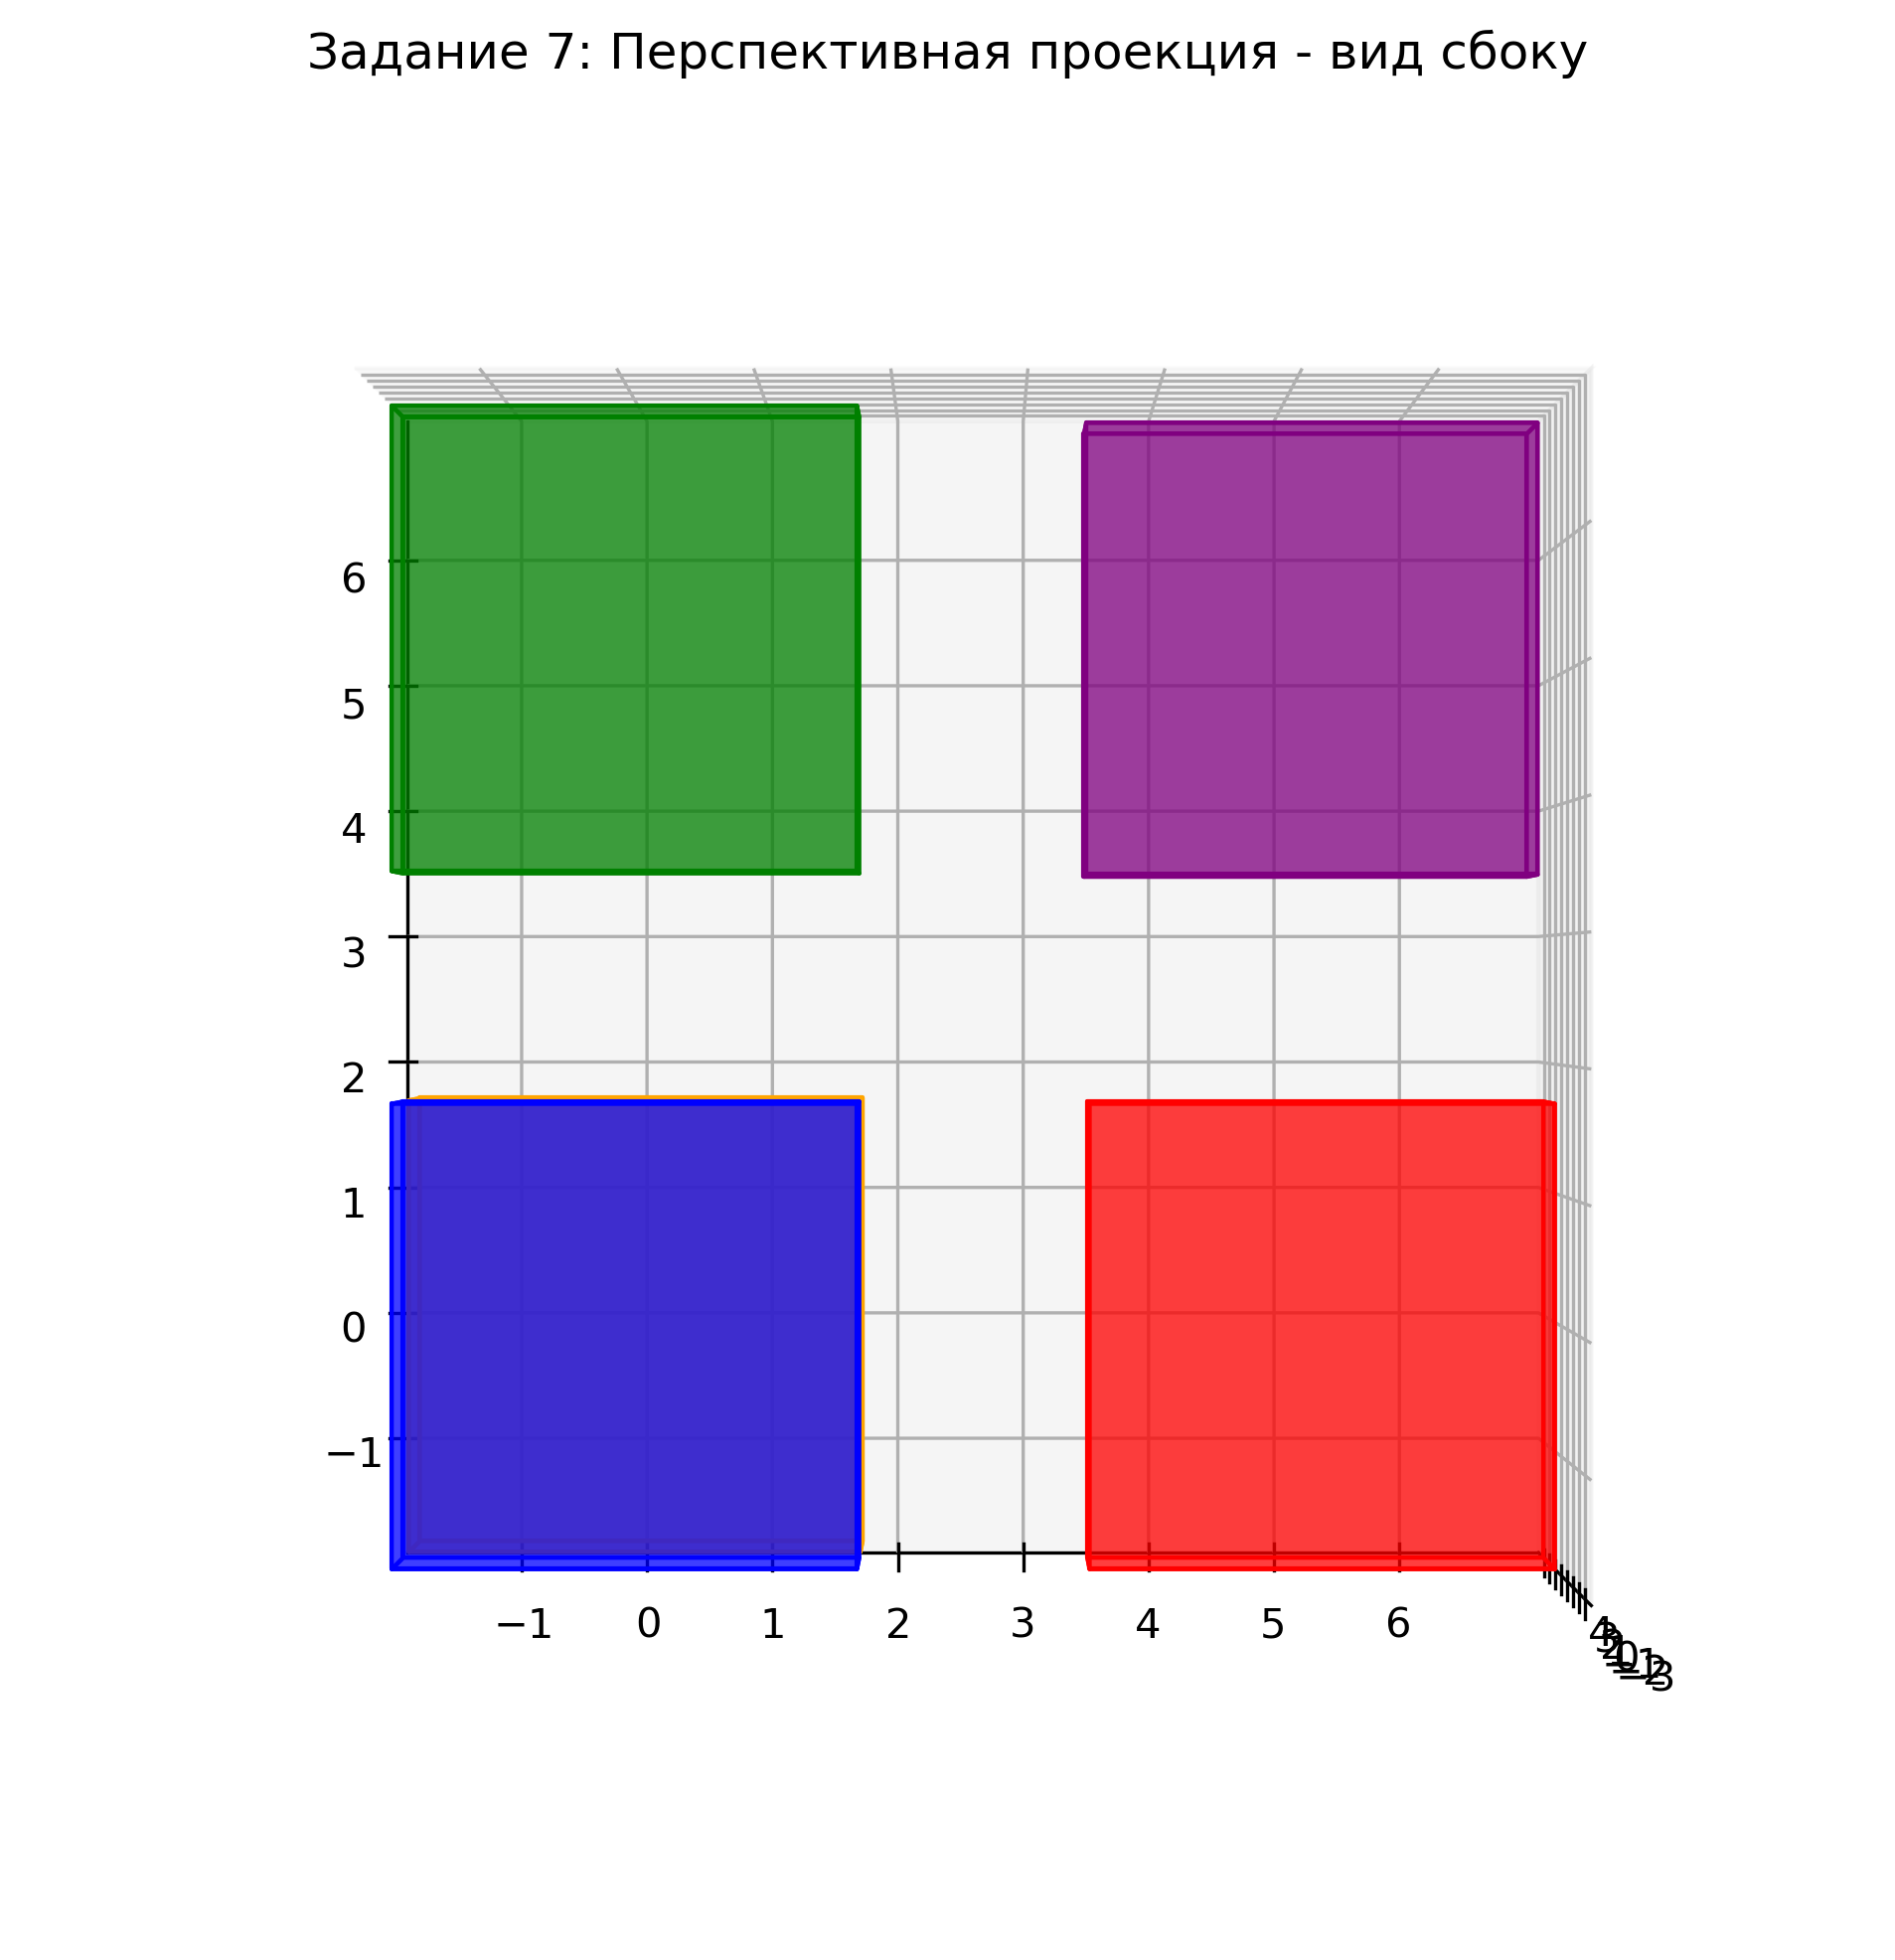
\includegraphics[width=0.6\textwidth]{task7/perspective_side_view.png}
    \caption{Задание 7: Перспективная проекция - вид сбоку для демонстрации эффекта перспективы}
\end{figure}

\textbf{Пояснения:}

Такая матрица позволяет корректно отображать удалённые объекты меньшими, чем ближние, и задаёт параметры видимости сцены (угол обзора, глубина, соотношение сторон).

\section{Выводы}

В ходе работы были реализованы и исследованы основные преобразования в 3D: масштабирование, перенос, поворот, а также перспективная проекция и виртуальная камера. Показано, как с помощью матриц можно гибко управлять положением и видом объектов в пространстве, а также формировать реалистичное изображение сцены.

\textbf{Ключевые результаты:}
\begin{itemize}
    \item Демонстрирована некоммутативность аффинных преобразований ($TS \neq ST$).
    \item Реализована формула Родрига для поворота вокруг произвольной оси.
    \item Показано, как комбинировать преобразования для сложных эффектов.
    \item Исследована перспективная проекция и её влияние на визуализацию 3D-сцен.
\end{itemize}
